% XCircuit output "dfe.tex" for LaTeX input from dfe.ps
\def\putbox#1#2#3#4{\makebox[0in][l]{\makebox[#1][l]{}\raisebox{\baselineskip}[0in][0in]{\raisebox{#2}[0in][0in]{\scalebox{#3}{#4}}}}}
\def\rightbox#1{\makebox[0in][r]{#1}}
\def\centbox#1{\makebox[0in]{#1}}
\def\topbox#1{\raisebox{-0.60\baselineskip}[0in][0in]{#1}}
\def\midbox#1{\raisebox{-0.20\baselineskip}[0in][0in]{#1}}
   \scalebox{0.951219}{
   \normalsize
   \parbox{6.83333in}{
   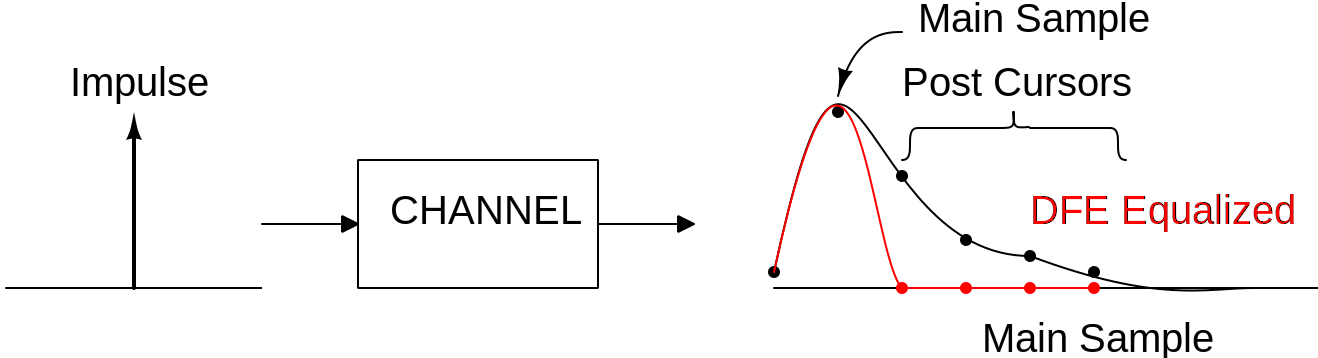
\includegraphics[scale=1.05128]{dfe}\\
   % translate x=937 y=-1 scale 0.36
   \putbox{5.14in}{0.09in}{1.20}{Main Sample}%
   \putbox{2.05in}{0.75in}{1.20}{CHANNEL}%
   \putbox{4.80in}{1.75in}{1.20}{Main Sample}%
   \putbox{4.72in}{1.42in}{1.20}{Post Cursors}%
   \putbox{0.39in}{1.42in}{1.20}{Impulse}%
   } % close 'parbox'
   } % close 'scalebox'
   \vspace{-\baselineskip} % this is not necessary, but looks better
